\documentclass[9pt,twocolumn,twoside]{osajnl}
%% Please use 11pt if submitting to AOP
% \documentclass[11pt,twocolumn,twoside]{osajnl}

\journal{ol} % Choose journal (ao,jocn,josaa,josab,ol,optica,pr)

%See template introduciton for guidance on setting shortarticle option
\setboolean{shortarticle}{false}
% true = letter/tutorial
% false = research/review article
% (depending on journal)

\usepackage{dblfloatfix}    % To enable figures at the bottom of page
\usepackage{amsmath}
\usepackage{mathrsfs}
\usepackage{float}
\floatstyle{plain}
\restylefloat{figure}


\title{Automating Instruments to Characterize Infrared Laser Diodes}

\author[1]{Jin Kiatvongcharoen}
\author[2]{Sam Schonsberg}

\affil[1,2]{Knight Campus Graduate Internship Program, University of Oregon, Eugene, OR 97403}
\affil[1]{jkiatvon@uoregon.edu}
\affil[2]{sschons2@uoregon.edu}


\begin{abstract}
Using the Python package PyVISA, we used a computer to automate the characterization of nLight laser diodes (LD) by interfacing with a source/measure unit and a digital multimeter. Characteristic current-voltage and current-light curves (IVL curves) of a LD at varying cavity lengths and temperatures were used to calculate various characteristic parameters of LDs. In addition, we manually examined the spectral characteristics of LD emission at different injection currents using a spectrometer to measure peak wavelengths of emission and the width (FWHM) of the peaks. Threshold currents and characteristic temperatures were accurately measured, but efficiency percentages and optical loss values were calculated with large error due to miscalculations within the data analysis. Nevertheless, we successfully demonstrated the characterization of LDs through a computer automation.
% Using the Python package PyVISA, we used a computer to automate the characterization of nLight laser diodes (LD) by interfacing with a source/measure unit and a digital multimeter. Characteristic current-voltage and current-light curves (IVL curves) of a LD were used to calculate various characteristic parameters of LDs, including the threshold current, differential quantum efficiency, wall plug efficiency, and series resistance. By collecting IVL curves for two LDs of different cavity lengths at different temperatures, the net internal optical loss, injection efficiency, and characteristic temperature of the LD material can also be calculated. In addition, a spectrometer was used to examine the spectral characteristics of LD emission at different injection currents, including the peak wavelength of emission and the width (FWHM) of the peak. Threshold currents and characteristic temperatures were accurately measured, but efficiency percentages and optical loss values were calculated with large error due to miscalculation within data analysis. 
\end{abstract}

\setboolean{displaycopyright}{false}

\begin{document}
\maketitle
\raggedbottom


\section{Introduction}
\indent \indent Automating technical processes is dominating industries all over the world. Automation becomes critical when an industry requires precise quality control of mass-produced products. In addition to shortening production time, automating systems and procedures significantly reduces human error and provides traceable feedback. If the procedure is standardized, the programmable software can become universal and benefit companies across the world. Examples of this include automating car production, analyzing data sets from large surveys, and assuring quality of semiconductor microchips. To explore the benefits of automation within the optics industry, we created an automation process to characterize nLight laser diodes. The procedure investigated the Python package PyVISA to interface with a source/measure unit and a digital multimeter in order to create IVL characteristic curves, from which various characteristics of the laser diode can be calculated.


\section{Background}

\indent \indent Laser diodes (LD) are similar to light-emitting diodes (LED), in which p-type and n-type doped semiconductors create light when pumped directly with electrical current. The applied current forces electrons from the n-type material to combine with holes from the p-type material, creating light. But, in the case of a LD, the two ends of the semiconductor are cleaved, forming very smooth perpendicular faces. This boundary between the semiconductor and air acts as a mirror via Fresnel reflection, so that a semiconductor cleaved at both ends acts as a planar mirror resonator cavity. In addition, the semiconductor material acts as a gain medium, allowing light amplification by stimulated emission of radiation. It is also common for LDs to have an i-type (i.e., intrinsic, or undoped) semiconductor layer sandwiched between the p-type and n-type doped semiconductor regions; this additional layer acts to confine the region where electrons and holes recombine to emit radiation. The i-type may also confine some radiation due to differences in index of refraction, which aids in the laser action within the diode \cite{Coldren}.

\begin{figure}[H]
\centering
\includegraphics[width=1\linewidth]{laser_diode_schematic.png}
\caption{\textbf{LD Schematic.} A schematic diagram of a typical LD. The LD is composed of an intrinsic (undoped) semiconductor sandwiched between p-type and n-type semiconductor layers. A current is applied across the diode which produces stimulated emission when the injection current is above a threshold value. Note the elliptical beam shape emitted by the LD due to light diffracting out of the opening face.}
\label{fig:LD_schematic}
\end{figure}

Current injected into the diode initially results in spontaneous emission similar to an LED. As the injection current increases, the amount of spontaneous emission increases as well; however, beyond a certain threshold current $I_{th}$, the amount of spontaneous emission reaches a maximum, and any further spontaneous emission triggers stimulated emission. It is at this point that the pumping of electrons by the applied current matches the losses in the cavity. The net optical loss in the cavity is described by the parameter $\langle \alpha_i \rangle$. Beyond $I_{th}$, light emitted by the diode is dominated by stimulated emission, hence the name laser diode. As injection current increases beyond $I_{th}$, the power output of the laser is linear as a function of current. This linear trend beyond $I_{th}$ is called the slope efficiency of the LD \cite{Coldren}.

The slope efficiency is indicative that the ratio between the photons out of the LD and the electrons pumped into the LD is constant; this is the differential quantum efficiency $\eta_d$, the number of photons out per electrons pumped in. It has been assumed thus far that all electrons pumped contribute to electron-hole recombination, but this is of course not the case. In reality, only a fraction of pumped electrons contribute to stimulated emission; this fraction is called the injection efficiency $\eta_i$ of the LD. The last type of efficiency to be considered is the so-called wall plug efficiency $\eta$, which is the ratio between the power out of the LD and the electrical power sent into the LD \cite{Coldren}.

Two final LD characteristics are the series resistance and the characteristic temperature. The series resistance $R_S$ is a measure of the quality of the metal contacts deposited onto the LD; a lower $R_S$ means current can flow more easily through the LD \cite{Kamran}. Since the material properties of the LD change with temperature, so too does $I_{th}$. Specifically, an increase in temperature decreases $\eta_i$ due to an increase in current leakage. Hence, a larger $I_{th}$ is necessary to overcome increased current leakage at higher temperatures. The dependence of $I_{th}$ on temperature is characterized by the characteristic temperature $T_0$ of the LD. A smaller $T_0$ results in $I_{th}$ having a more sensitive temperature dependence \cite{Coldren}.

All of the above parameters are explained in mathematical detail in the appendix \textbf{Section C}.

\section{Experiment/Method}
\indent \indent Two key pieces of information to characterize laser diodes (LDs) are the diode's characteristic current-voltage (IV) and current-light (IL) curves (collectively, IVL curves) \cite{Coldren}. These graphically display the LD injection current as a function of the voltage across the diode and the power out of the LD as a function of the injection current respectively (see \textbf{Fig. \ref{fig:IV}} and \textbf{Fig. \ref{fig:IL}}). From these three sets of data (injection current, LD voltage, and LD power), quantities such as the series resistance, threshold current, differential quantum efficiency, and wall plug efficiency can be calculated for a particular LD (see \textbf{Table \ref{tab:Characteristics1}}). If IVL measurements are taken for two LD cavity lengths at two different temperatures, additional quantities such as net internal optical loss, injection efficiency, and characteristic temperature can be calculated, provided the two LDs are physically identical apart from cavity length (see \textbf{Table \ref{tab:Characteristics2}}).

In addition to the above values, one can also examine the spectral output of the LD as a function of injection current, including peak emission wavelength and the full-width at half-maximum (FWHM) of the peak (see \textbf{Fig. \ref{fig:spectra}} and \textbf{Table \ref{tab:Characteristics1}}).

An automated data collection process allows IVL data sets to be recorded in approximately 15 minutes depending on the size of the current step increment, which is much quicker and more consistent between data sets than if each data set were recorded by hand. In order to automate IVL curve data collection, the setup shown in \textbf{Fig. \ref{fig:schematic}} was used. A computer connected via USB to an SMU and DMM records current injected into the LD via the SMU, voltage across the LD via the SMU, and voltage out of the photodiode (PD) via the DMM (note that this voltage is originally a current output by the PD which is converted into a voltage by a 1 kΩ current-voltage converter). The LD's temperature is held nearly constant by a thermoelectric cooler (TEC) which is controlled by the TEC Controller whose controls are set manually. Light emitted by the LD enters an integrating sphere, which evenly spreads the incident beam's power across the inner surface of the sphere, minimizing any spatial distribution of the emitted light and allowing for a simpler method of capturing most of the output power.

\begin{figure}[H]
\centering
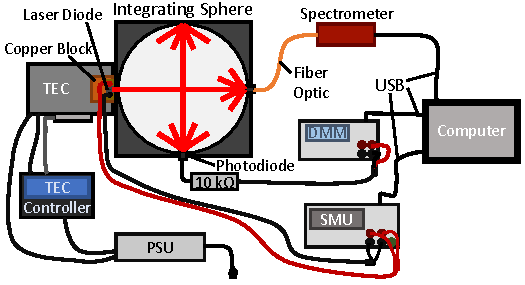
\includegraphics[width=1\linewidth]{schematic}
\caption{\textbf{Experimental Setup.} The experimental setup for automating laser diode characterization. A computer communicates to a source/measure unit (SMU), digital multimeter (DMM), and spectrometer via USB connections. The Python module PyVISA was used to send SCPI commands to the SMU and DMM in order to inject pulses of current into the laser diode (LD), measure the resultant voltage across the LD, and measure the voltage output by the photodiode (originally a current which is converted to a voltage by a load resistor of 1 k$\Omega$). The temperature of the laser diode is held fairly constant by a thermoelectric cooler (TEC) controlled by a TEC Controller. The integrating sphere spreads input laser light evenly across the inner surface of the sphere, allowing the power output by the LD to be calculated from the power measured by the photodiode (see \textbf{Eqns. 8, 9, 10}).}
\label{fig:schematic}
\end{figure}

In addition, the computer is connected to a spectrometer to record spectral composition of the LD output light at currents below, at, and above the threshold current; note that spectra were recorded manually because of a lack of time to fully automate the spectrometer. See the appendix \textbf{Section A} for more detailed information on the equipment used in this experiment. See \textbf{Fig. \ref{fig:spectra}} for typical LD spectra as a function of injection current, and see the appendix \textbf{Section B} for more detailed supplementary spectra.

In order to interface with the SMU and DMM, commands using syntax of standard commands for programmable instruments (SCPI) were converted to machine-level code by the Python package PyVISA. In other words, instrument commands were written in Python code which was executed and translated to commands which the instruments could understand and perform. SCPI commands were found in programming guides for the SMU and DMM \cite{SMUprogramguide,DMMprogramguide}. Data sets were recorded as .csv files and analyzed in a separate Python script.

To form our IVL data sets, we measured values for injection currents of 0 A up to 2 A in steps of 0.01 A. At each injection current value, 2000 pulses of 500 $\mu$s width were sent to the LD. For each pulse, the SMU was instructed to wait 450 $\mu$s before making a measurement with a 50 $\mu$s aperture time. The average of the 2000 measurements for the injection current and voltage across the LD was recorded, and the process was repeated for the next step in injection current values. During each train of pulses, the DMM was instructed to make five voltage measurements, each spaced by 50 ms; the average of these five measurements was recorded for each step in injection current.

Choosing the above pulse and measurement timing parameters was done over a period of two weeks of trial and error and manual optimization of the SMU and DMM. A pulse width of 500 $\mu$s allows the SMU enough time to ramp up to an output of 2 A and maintain the peak current for at least 50 $\mu$s at the end of the pulse, hence the measurement delay of 450 $\mu$s and the aperture time of 50 $\mu$s. The pulse width was set as small as possible to avoid possible heat issues with the LD (this allowed us to assume the LD was at a constant temperature reported by the TEC Controller). The parameters for the DMM were manually optimized to return the highest voltage out of the PD possible (corresponding to the peak output of the laser diode during the current pulse train).


\section{Results}
\indent \indent After successfully interfacing with the SMU and DMM, we characterized the laser diode by analyzing IV and IL curves for each unique combination of cavity lengths and temperatures. \textbf{Fig. \ref{fig:IV}} and \textbf{Fig. \ref{fig:IL}} displayed the measured results after applying pulses of increasing currents through each laser diode. 

\begin{figure}[htbp]
\centering
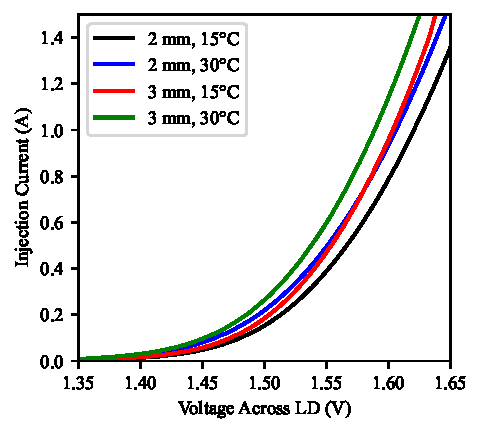
\includegraphics[width=0.95\linewidth]{IVcurve}
\caption{\textbf{IV Curve.} IV characteristic curves of each respective laser diode with the injection current (A) plotted against the voltage (V) across the laser diode (LD), both measured from the SMU. Each laser diode possessed non-ohmic behavior, where longer cavity length LDs reached peak values at a faster rate than shorter LDs. For both lengths, the increase in temperature delayed ramp-up time and resulted in larger voltages. Plot focused within 1.35-1.65 V range. \textbf{Fig. \ref{fig:IVfull}} displays the entire data set.}
\label{fig:IV}
\end{figure}

The IV curve for each configuration of laser diodes displayed non-ohmic behavior, as each curve increased non-linearly as the applied current grew larger. \textbf{Fig. \ref{fig:IV}} also demonstrated the behavior of the voltage response when varying cavity lengths and temperatures. As the cavity length increased from 2 mm to 3 mm, the voltage across the diode decreased by a factor of 1\%. Similarly, when the temperature increased from 15°C to 30°C, the voltage across the diode decreased by a similar amount. 

\begin{figure}[hbtp]
\centering
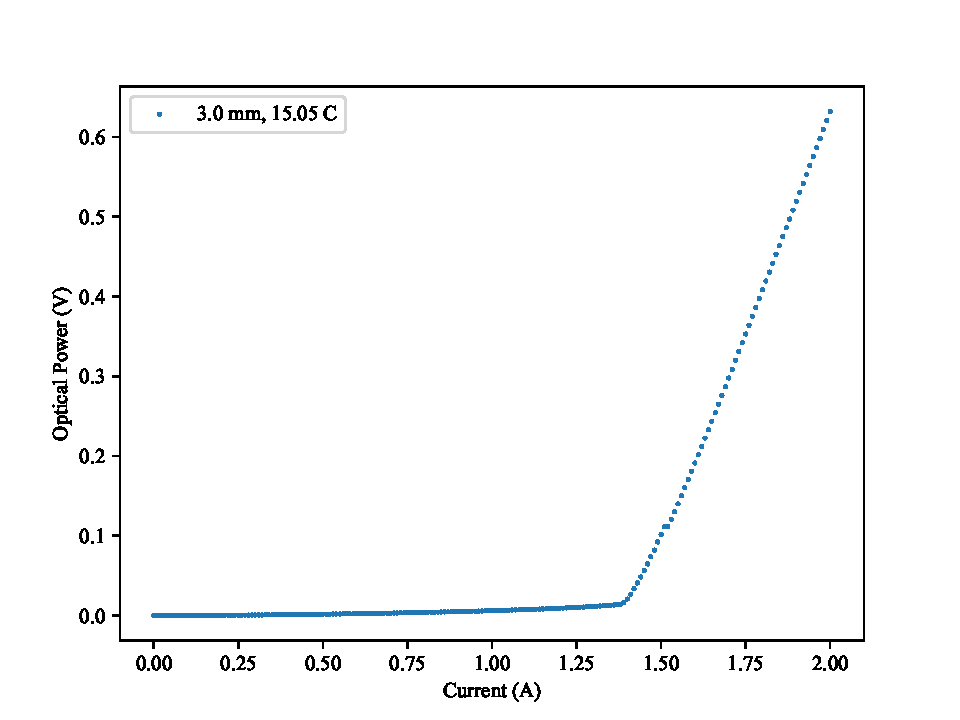
\includegraphics[width=0.95\linewidth]{ILcurve}
\centering
\caption{\textbf{IL Curve.} IL characteristic curves with the injection current (A) plotted against the power (W) out of the laser diode (LD), where the luminosity is calculated from converting voltage readings from photodetector in integrating sphere to output power of the LD. Threshold currents, $I_{th}$, and differential quantum efficiencies, $\eta_d$, displayed in \textbf{Table 1.} in appendix \textbf{Section C}. Based on magnitude of slopes, the longer cavity length LDs portrayed higher efficiency, where an increase in temperature delayed lasing currents.}
\label{fig:IL}
\end{figure}

Unlike the IV curve, the IL curve in \textbf{Fig. \ref{fig:IL}} was initially measured in volts from the DMM, from which was then converted into power using the calculations from the appendix \textbf{Section C. Integrating Sphere Theory}. The IL characteristic curves most notably displayed the actual lasing of the laser diode and their corresponding threshold currents. Methodology for solving threshold currents and efficiency parameters are shown in appendix \textbf{Section C}. From our measurements, the longer cavity length LDs exhibited shorter threshold currents with larger slope efficiencies. The temperature also only seemed to affect the threshold currents, as the slope efficiencies remained very similar at varying temperatures. 

Alongside the IVL characteristics, we collected spectra data for each configuration of laser diodes to display the emission behavior before, at, and after threshold current. \textbf{Fig. \ref{fig:spectra}} displayed the emitted spectra for the L = 3 mm and T = 30°C laser diode with an offset between each spectra and normalized units. As expected, the laser diode exhibited a wavelength spectra similar to an LED before threshold current and gradually revealed lasing behavior after enough current was injected to pass the threshold. 


\begin{figure}[hbtp]
\centering
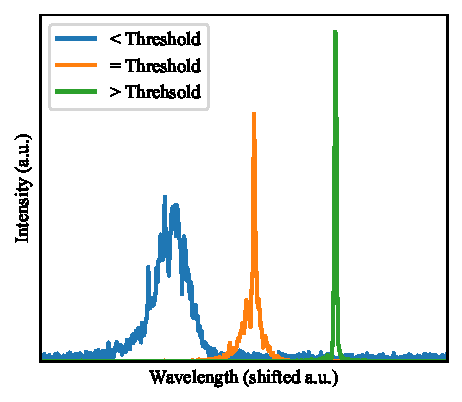
\includegraphics[width=0.95\linewidth]{Example_Spectra}
\caption{\textbf{Spectra.} Typical spectra emitted by a laser diode (LD) below, at, and above the threshold current. Note that emission line centers have been shifted to display differences in linewidth, and intensity is normalized to display qualitative differences in output intensity. Below threshold, the width of LD emission is comparable to an LED. As the current apporoaches the threshold value, stimulated emission begins to dominate LD output, reflected by the narrowing of the emission line. Above threshold, the line narrows even further, and the slight ``wings" on either side at threshold disappear.}
\label{fig:spectra}
\end{figure}

\textbf{Fig. \ref{fig:SerRes}} displayed the series resistance curve, in addition to the IV curve from \textbf{Fig. \ref{fig:IV}} with swapped axis. The series resistance behaved consistently with theoretical work from \cite{paul}.

\begin{figure}[hbtp]
\centering
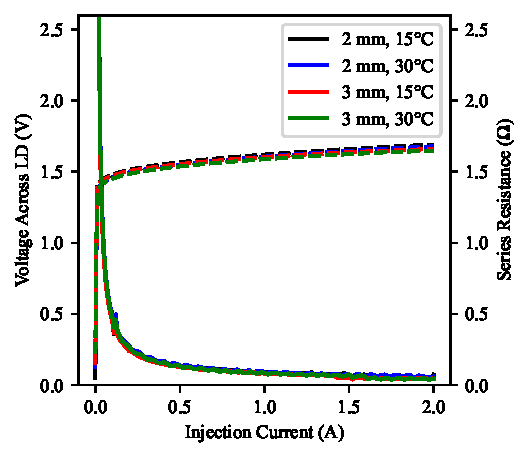
\includegraphics[width=1\linewidth]{SeriesRes}
\caption{\textbf{Series Resistance.} Dual plot of the laser diode (LD) voltage and the series resistance plotted against injection current. The series resistance (given by $R_S = \frac{dV}{dI}$) is a measure of the quality of the metal contacts deposited on the LD (CITE). There is a clear decreasing trend, i.e., the series resistance decreases as injection current increases. Beyond the threshold current, $R_S$ for the 2mm and 3mm diodes is roughly 0.06 Ω and 0.04 Ω respectively.}
\label{fig:SerRes}
\end{figure}

All extra plots, such as the raw data plots for the IVL curves, characteristic temperature plot, inverse differential quantum efficiency plot, and emission spectrum data for each LD, were shown in appendix \textbf{Section B.}. Further analysis for each characterization parameter were shown in appendix \textbf{Section C.}, and final results were displayed in \textbf{Tables \ref{tab:Characteristics1} \& \ref{tab:Characteristics2}}.



\section{Discussion}

\indent \indent With our automated procedure, the IVL characteristics followed expected behavior for each individual laser diode. \textbf{Fig. \ref{fig:IV}} correctly displayed the non-ohmic behavior of semiconductor diodes, while \textbf{Fig. \ref{fig:IL}} showed appropriate threshold currents with a linear trend when lasing. However, the data collection process and characterization analysis still suffered from several faults.  

The first inconsistency within our data regarded the relationship between different length diodes and their output power slope efficiencies. Theoretically, Larger length diodes should possess greater power loss due to the increased length electrons need to travel to emit stimulated emission. However, \textbf{Fig. \ref{fig:IL}} displayed the 3 mm length diode producing larger power output with a stronger slope efficiency compared to the 2 mm diode. This poor characterization caused the analysis for the net optical loss, $\langle \alpha_i \rangle$, and injection efficiency, $\eta_i$, to be nonsensical, as shown in \textbf{Table \ref{tab:Characteristics2}}. With this unexpected result, we characterized a 1.5 mm laser diode to investigate this inconsistency with theory and whether this trend followed for a shorter cavity length. \textbf{Fig. \ref{fig:QuantEff}} in the appendix \textbf{Section B} displayed the inverse differential quantum efficiency of all three diodes after collecting the appropriate data and showed the trends between lengths. The negative correlation between 2 mm and 3 mm represented the inconsistency with theory, while the positive correlation between 1.5 mm and 2 mm displayed the expected behavior of a more efficient diode for the shorter cavity length. This inferred that the 3 mm data defected the characterization of the laser diode we assumed to be consistent for all three cavity lengths. Because of this, we suspected that the 3 mm diode must be physically different compared to the other two. This difference could stem from an overlooked reflective coating in the cavity or a change in semiconductor material that exhibited different lasing behaviors. Nevertheless, this investigation pinpointed one of the sources of errors within the analysis and displayed the advantages of our automated procedure due its ability to quickly characterize the 1.5 mm laser diode. 

The final hiccup that disoriented the data analysis was the conversion of DMM voltage readings to the actual power output of the laser diode. As shown in \textbf{Fig. \ref{fig:IL}}, the max output power was recorded to be 0.10 W over 0.6 A of current from the L = 3 mm laser diode at T = 15°C. This produced a slope efficiency of approximately 10\%, which compared poorly to accepted data that measured efficiencies within the magnitude of 90\% \cite{paul}. We attributed this to the data analysis when incorporating the integrating sphere theory from appendix \textbf{Section C.} If more time was provided, we would further investigate this area of the data analysis and study higher-detailed literature to find the sources of our miscalculations.



\indent \indent 

\section{Conclusion}

\indent \indent The automation process for characterizing a laser diode proved successful with its ability to quickly run 2000 pulses for each increasing injection current and measure their corresponding voltage and power output values. The usage of SCPI commands and the PyVISA library allowed us to flexibly control the SMU and DMM in accordance with one another and optimize pulse settings to ensure proper heat management within each laser diode. Despite the mathematical errors when calculating the various parameters, we effectively constructed a coded automation that collected IVL characteristics for a given laser diode and found their respective threshold currents and characteristic temperatures. Further improvements to data analysis procedures would include a deeper dive into literature, better utilization of integrating sphere theory, and perhaps an automated procedure for emission spectra data. Nevertheless, this new procedure of automating instrumentation to characterize a laser diode demonstrated its ability to significantly reduce manual labor time and eventually destroy the human race as we know it. 


\section*{Acknowledgement}
\indent \indent We would like to acknowledge the Knight Campus Graduate Internship Program for providing the idea of this experiment and all of its necessary supplies and equipment. 

We would also like to acknowledge Erik Keever for his expertise and guidance when we were in desperate need of help and felt extremely lost.

A special thank you to the best track director Nima Dinyari for his motivational speeches and boost in morale, and a overall thank you to all the colleagues that kept our sanity in check.

Lastly, we would like to give a special thanks to the submarine alarm stock sound that we included at the beginning of our code for making our measuring procedure enjoyable to execute.


% \cite{Coldren}
% \cite{durell}
% \cite{ThorlabsPD}
% \cite{SMU}
% \cite{SMUprogramguide}
% \cite{DMM}
% \cite{DMMprogramguide}
% \cite{PSU}
% \cite{TEC}
% \cite{Peltier}
% \cite{IntSphere}
% \cite{Spectrometer}
% \cite{Kamran}

% Bibliography
\bibliography{sample}
\bibliographystyle{unsrt}

\newpage
\clearpage

\appendix
\section*{APPENDIX}

\section{Equipment Used}
The following is a list of equipment used in this experiment:
\begin{itemize}
    \item Keysight B2901A Source/Measure Unit \cite{SMU}
    \item Rigol DM3068 6 1/2 Digit Digital Multimeter \cite{DMM}
    \item Mean Well RSP-320-24 Power Supply Unit \cite{PSU}
    \item TE Technology CP-061HT Cold Plate Cooler \cite{Peltier}
    \item TE Technology TC-720 Thermoelectric Temperature Controller \cite{TEC}
    \item nLight Laser Diodes (1.5mm, 2mm, 3mm cavity lengths)
    \item Thorlabs IS236A-4 2", 4-Port, Integrated Photodiode Integrating Sphere \cite{IntSphere}
    \item Thorlabs SM05PD1B Photodiode (integrated into integrating sphere) \cite{ThorlabsPD}
    \item Thorlabs CCS175 Spectrometer \cite{Spectrometer}
\end{itemize}

\section{Supplemental Plots}


\begin{figure}[H]
\centering
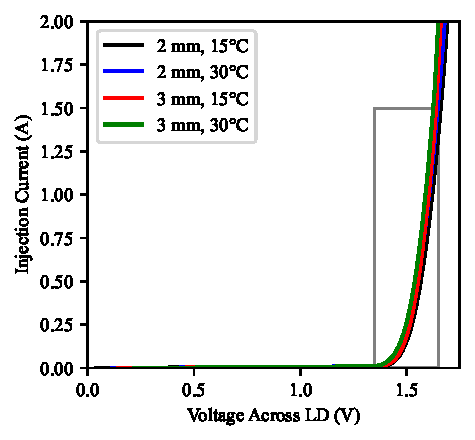
\includegraphics[width=1\linewidth]{IVcurveFull}
\caption{\textbf{Full IV Curve.} Full data set for IV characteristic curves of 2 mm and 3 mm LDs at T = 15°C and T = 30°C. The nonlinear relation between I and V displays the non-ohmic properties of laser diodes.}
\label{fig:IVfull}
\end{figure}

\begin{figure}[H]
\centering
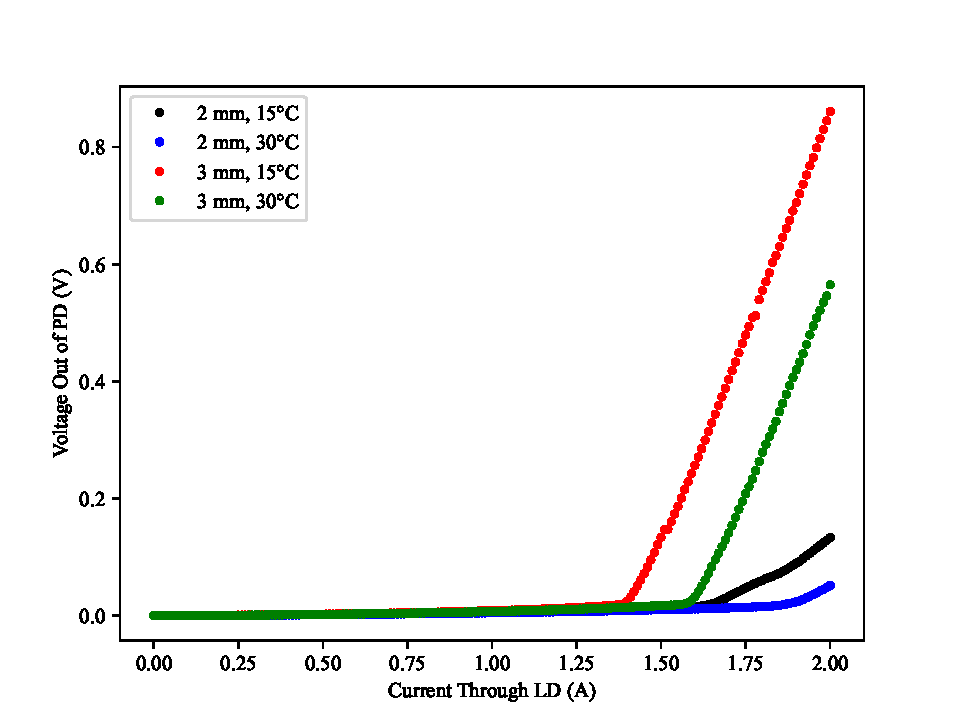
\includegraphics[width=1\linewidth]{ILcurveVolt}
\caption{\textbf{Full IL Curve.} Raw data set for IL characteristic curves of L = 2 mm, 3 mm at T = 15°C, 30°C. Injection current (A) plotted against voltage (V) out of the photodetector (PD) inside integrating sphere.}
\label{fig:ILfull}
\end{figure}

\begin{figure}[H]
\centering
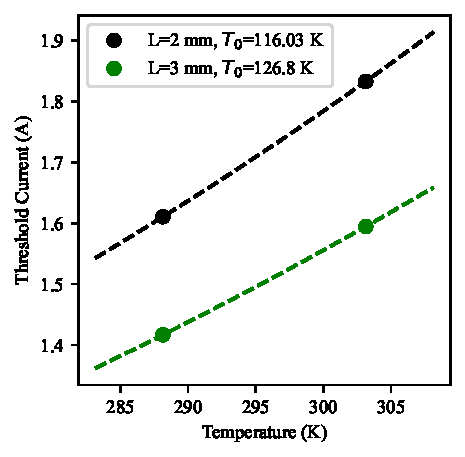
\includegraphics[width=1\linewidth]{ThresholdCurrent}
\caption{\textbf{Characteristic Temperature} Plot of threshold current as a function of the temperature of the laser diode. The threshold current for both laser diode lengths increases with temperature as described by \textbf{Eqn. 7}, where the characteristic temperature $T_0$ is shown in the plot legend.}
\label{fig:CharTemp}
\end{figure}

\begin{figure}[H]
\centering
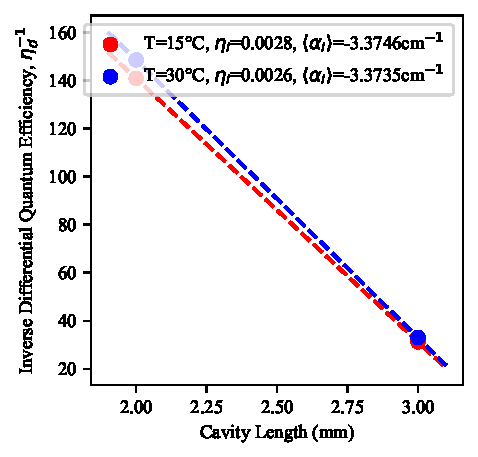
\includegraphics[width=1\linewidth]{DiffQuantEff}
\caption{\textbf{Inverse Efficiency vs. Length.} Dual plot of $\eta_d^{-1}$ vs. L for combinations L = 2-3 mm and L = 1.5-2 mm, where red and blue corresponds to T = 15°C and T = 30°C, respectively. Negative trend for L = 2-3 mm opposes theory and suggests a misassumption about 3 mm laser diode. We suspect a physical difference in material or unique reflective coating within resonator cavity that differs from 1.5 mm and 2 mm laser diode.}
\label{fig:QuantEff}
\end{figure}


\begin{figure}[H]
\centering
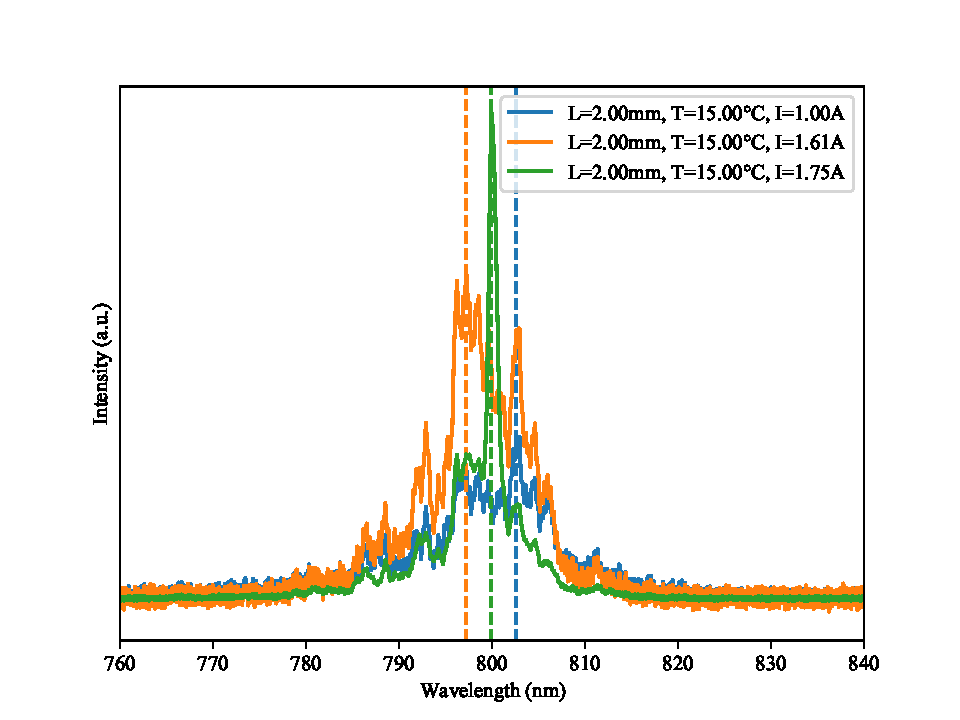
\includegraphics[width=1\linewidth]{Spectra_2.00_15.00.pdf}
\caption{\textbf{Spectra for L = 2 mm, T = 15°C.} Emission spectra for the 2mm laser diode at 15°C for currents below, at, and above threshold current. Specific currents for each spectrum are given in the plot legend; peak wavelengths are marked by vertical dashed lines.}
\label{fig:false-color}
\end{figure}



\begin{figure}[H]
\centering
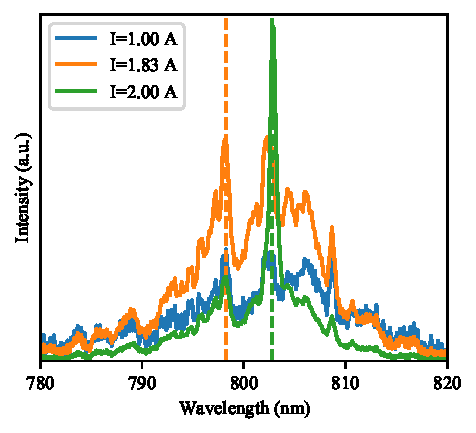
\includegraphics[width=1\linewidth]{Spectra_2.00_30.00.pdf}
\caption{\textbf{Spectra for L = 2mm, T = 30°C.} Emission spectra for the 2mm laser diode at 30°C for currents below, at, and above threshold current. Specific currents for each spectrum are given in the plot legend; peak wavelengths are marked by vertical dashed lines.}
\label{fig:false-color}
\end{figure}


\begin{figure}[H]
\centering
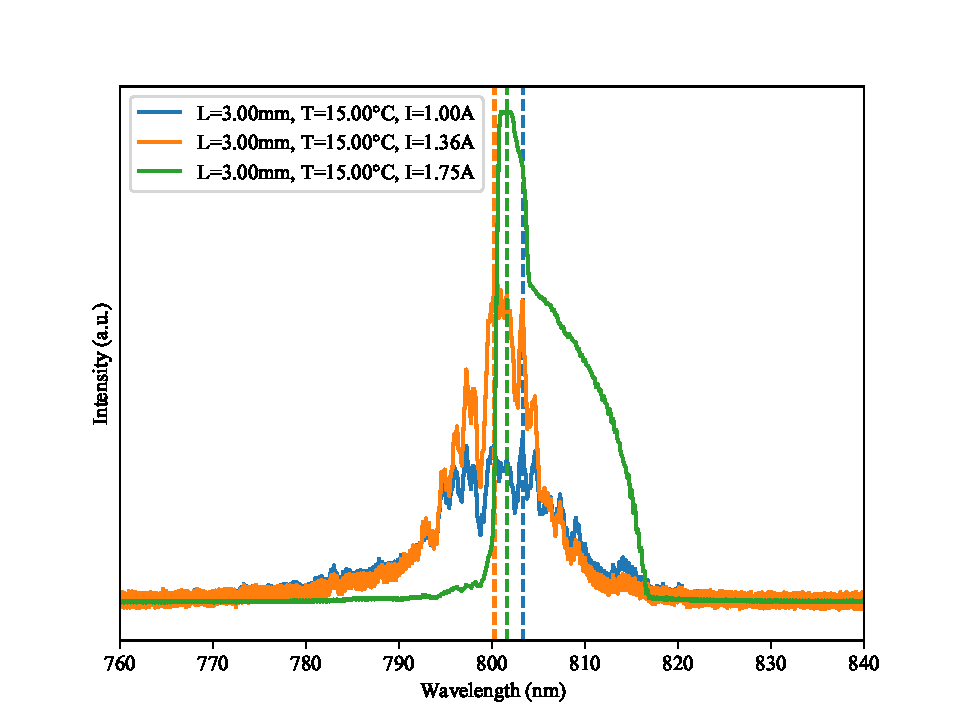
\includegraphics[width=1\linewidth]{Spectra_3.00_15.00.pdf}
\caption{\textbf{Spectra for L = 3mm, T = 15°C.} Emission spectra for the 3mm laser diode at 15°C for currents below, at, and above threshold current. Specific currents for each spectrum are given in the plot legend; peak wavelengths are marked by vertical dashed lines.}
\label{fig:false-color}
\end{figure}

\begin{figure}[H]
\centering
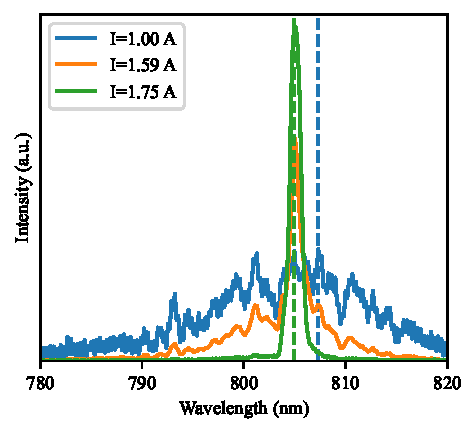
\includegraphics[width=1\linewidth]{Spectra_3.00_30.00.pdf}
\caption{\textbf{Spectra for L = 3mm, T = 30°C.} Emission spectra for the 3mm laser diode at 30°C for currents below, at, and above threshold current. Specific currents for each spectrum are given in the plot legend; peak wavelengths are marked by vertical dashed lines.}
\label{fig:false-color}
\end{figure}

\section{Calculations \& Results}

\begin{table*}[!t]
\centering
\begin{tabular}{|c |c|c|c| c|}
\hline
 & L = 2 mm, T = 15$^o$C & L = 2 mm, T = 30$^o$C & L = 3 mm, T = 15$^o$C & L = 3 mm, T = 30$^o$C \\
\hline\hline
$I_{th}$ & 1.61 A & 1.83 A & 1.42 A & 1.59 A \\
\hline
$\eta_d$ & 2.42\% & 2.29\% & 10.88\% & 10.29\% \\
\hline
$\eta (I=2$A) & 0.5\% & 0.2\% & 3\% & 2\% \\
\hline
$R_S (I>I_{th})$ & 0.06 Ω & 0.06 Ω & 0.045 Ω & 0.045 Ω \\
\hline
$\lambda (I < I_{th})$ & 802.62 nm & 798.25 nm & 803.29 nm & 807.32 nm \\
\hline
$\lambda (I \approx I_{th})$ & 797.25 nm & 798.25 nm & 801.61 nm & 804.97 nm \\
\hline
$\lambda (I > I_{th})$ & 798.25 nm & 802.78 nm & 801.95 nm & 804.97 nm \\
\hline
$\Delta\lambda (I < I_{th})$ & 13.59 nm & 14.6 nm & 13.76 nm & 19.98 nm \\
\hline
$\Delta\lambda (I \approx I_{th})$ & 11.91 nm & 13.26 nm & 5.2 nm & 1.34 nm \\
\hline
$\Delta\lambda (I > I_{th})$ & 1.17 nm & 0.84 nm & 1.68 nm & 1.18 nm \\
\hline
\end{tabular}
\centering
\caption{\textbf{Individual LD Characteristics}. Measured/calculated characteristic quantities for individual LDs of a given length at a given temperature. Includes threshold current ($I_{th}$), differential quantum efficiency ($\eta_d$), wall plug efficiency at 2 A ($\eta$), series resistance above the threshold current ($R_S$), peak wavelength at a given current ($\lambda$), and the full-width at half-maximum (FWHM) of the peak emission line of the LD at a given current ($\Delta \lambda$).}
\label{tab:Characteristics1}
\end{table*}





\subsection*{Threshold Current, $I_{th}$}
\indent \indent Threshold currents, $I_{th}$, were measured by fitting a linear regression on \textbf{Fig. \ref{fig:IL}} using all the data points after the LD started lasing and calculating the x-intercept at which the best-fit lines crossed 0 W power. We manually counted the point at which the diode started lasing for each configuration of LD. 

\subsection*{Differential Quantum Efficiency, $\eta_d$}
\indent \indent After solving the threshold currents for each LD, the differential quantum efficiencies were solved by using the following equation \cite{Coldren}:
\begin{equation}
    \eta_d=\frac{q}{h\nu}\frac{dP_{0}}{dI} \,,
\end{equation}
where $q$ is the charge of an electron, $h$ is Planck's constant, $\nu$ is the frequency of light, and $\frac{dP_0}{dI}$ is the magnitude of the linear regression after lasing.

\subsection*{Wall Plug Efficiency, $\eta$}
\indent \indent Wall plug efficiency was calculated as the ratio of the optical power out of the LD divided by the electrical power into the LD:
\begin{equation}
    \eta = \frac{P_0}{I V} \,,
\end{equation}
where $P_0$ is the power output by the LD, $I$ is the injection current, and $V$ is the voltage across the LD. The wall plug efficiency was current dependent, so the reported value is evaluated at maximum current, 2 A.

\subsection*{Series Resistance, $R_S$}
\indent \indent Series resistance is given by the derivative of the voltage across the LD with respect to the injection current:
\begin{equation}
    R_S = \frac{dV}{dI} \,,
\end{equation}
where $V$ is the voltage across the LD and $I$ is the injection current. Note that $R_S$ was found by numerical derivation. Also note that $R_S$ is highly variable with current, so the reported values are the average $R_S$ for currents above the threshold current.

\subsection*{Net Internal Optical Loss, $\langle \alpha_i \rangle$}
\indent \indent With $\eta_d$ known for each LD, the net internal optical loss and injection efficiency were calculated by plotting the inverse of $\eta_d$ against the cavity length $L$, shown in \textbf{Fig. \ref{fig:QuantEff}}. The linear regression between points would then follow the equation \cite{Coldren}:
\begin{equation}
    \frac{1}{\eta_d}=\frac{\langle \alpha_i \rangle}{\eta_i \ln{\left(\frac{1}{R}\right)}}L + \frac{1}{\eta_i} \,,
\end{equation}
where $R=r_1r_2$ is the total reflectivity of the mirrors in the cavity (it was assumed that $R=0.33$). If the linear regression from \textbf{Fig. \ref{fig:QuantEff}} followed the form $\eta_d^{-1}=mL+b$, then the net internal optical loss was calculated by
\begin{equation}
    \langle \alpha_i \rangle = m\eta_i \ln{\left(\frac{1}{R}\right)} \,.
\end{equation}

\subsection*{Injection Efficiency, $\eta_i$}
\indent \indent Similarly to $\langle \alpha_i \rangle$, the injection efficiency was calculated by plotting the linear regression in \textbf{Fig. \ref{fig:QuantEff}} and measuring the inverse of the y-intercept. That is,
\begin{equation}
    \eta_i = \frac{1}{b} \,.
\end{equation}

\subsection*{Characteristic Temperature, $T_0$}
\indent \indent With the threshold currents known for varying temperatures, the characteristic temperature was calculated using the equation
\begin{equation}
    I_{th}=I_0e^{T/T0} \,,
\end{equation}
where $I_0$ was an arbitrary constant term for the threshold currents. With two threshold currents and two temperatures, we were able to solve for the two unknowns, $I_0$ and $T_0$, apparent in the equation. 


\subsection*{Integrating Sphere Theory}
\indent \indent In order to quantify the power output of the LD, the voltage readings from the DMM must first convert back to the power received by the photodetector inside the integrating sphere. This conversion depends on the responsivity of the photodetector and the load resistance. That is \cite{ThorlabsPD},
\begin{equation}
    P_{PD}=\frac{V_0}{\mathcal{R}(\lambda)* R_L} \,,
\end{equation}
where $P_{PD}$ is the total power received by the photodetector, $V_0$ is the output voltage measured by the DMM, $\mathcal{R}(\lambda)$ is the wavelength-dependent responsivity of the detector material, and $R_L$ is the load resistance. For the SM05PD1B photodetector \cite{ThorlabsPD}, the responsivity at the wavelength for each laser diode (approximately $\lambda = 800$ nm) is $\mathcal{R}=0.5$ A/W. The load resistance was $R_L=1.086$ k$\Omega$. 

With the total power received by the photodetector, the output radiance, $L=\frac{P_{PD}}{A_{PD}}$, could then be derived to solve for the input flux of the LD by considering the reflectivity of the integrating sphere and the power loss from the other ports. This was derived from \cite{durell} and follows the equation
\begin{equation}
    L=\frac{P_{PD}}{A_{PD}}=\frac{\Phi}{A_S}M \,,
\end{equation}
where $A_{PD}$ is the area of the port for the photodetector, $\Phi$ is the input radiant flux (power from LD into the integrating sphere), $A_S$ is the surface area of the integrating sphere, and $M$ is the sphere multiplier, defined as
\begin{equation}
    M=\frac{\rho}{1-\rho(1-f)} \,,
\end{equation}
where $\rho$ is the reflectivity of the sphere coating ($\rho=99\%$) and $f$ is the port fraction defined as the ratio of the total area of non-reflective open ports over the surface area of the sphere. With dimensions taken from \cite{IntSphere, ThorlabsPD}, the input radiant flux (power out of LD into sphere), $\Phi$, was calculated and plotted as $P_0$ in \textbf{Fig. \ref{fig:IL}}.


\newpage

\begin{table}[H]
\centering
\begin{tabular}{|c |c|c|c| c|}
\hline
 & T = 15$^o$C & T = 30$^o$C & L = 2 mm & L = 3 mm \\
\hline\hline
$\langle \alpha_i \rangle$ & -3.37 cm$^{-1}$  & -3.37 cm$^{-1}$ & N/A & N/A \\
\hline
$\eta_i$ & 0.95\% & 0.9\% & N/A & N/A\\
\hline
$T_0$ & N/A & N/A & 116.03 K & 126.8 K \\
\hline
\end{tabular}
\centering
\caption{\textbf{Combined Characteristics}. Calculated characteristics requiring information from at least two LDs. Includes the net internal optical loss ($\langle \alpha_i \rangle$) and injection efficiency ($\eta_i$) which both require measurements of two LD lengths at the same temperature; also includes the characteristic temperature ($T_0$) which requires measurements of the same length LD at two different temperatures. Note that the calculated $\langle \alpha_i \rangle$ values are completely unphysical since the net internal optical loss will always be positive; this is due to the differential quantum efficiency of the longer (3mm) LD cavity length being higher than that of the shorter (2mm) LD. This leads to the conclusion that the two LDs tested were not physically identical apart from length (see \textbf{Sec. 5} and \textbf{Fig. \ref{fig:QuantEff}}).}
\label{tab:Characteristics2}
\end{table}



\end{document}